\documentclass[14pt,twoside,a4paper]{article}
\usepackage[slovak]{babel}
\usepackage{cite}
\usepackage[utf8]{inputenc}
\usepackage{graphicx}
\usepackage{url} % príkaz \url na formátovanie URL
\usepackage{hyperref}
\pagestyle{headings}

\title{Gamifikácia v informačných technológiach\thanks{Semestrálny projekt v predmete Metódy inžinierskej práce, ak. rok 2022/23, vedenie: Ing. Richard Marko, PhD.}}

\author{Leonid Gurulev\\[2pt]
	{\small Slovenská technická univerzita v Bratislave}\\
	{\small Fakulta informatiky a informačných technológií}\\
	{\small \text{qgurulev@stuba.sk}}
	}

\date{\small 30. december 2022}



\begin{document}


\maketitle
\begin{abstract}
Co tu pisat?
\end{abstract}

\section{Úvod}
V tomto článku sa budeme zaoberať možnosťami gemifikácie v oblasti informatiky, 
kde sa pridaním herných prvkov do štúdia a vývoja informačných technológií 
a programovania uľahčilo štúdium programovania a informatiky pre mnohých ľudí, 
rovnako, ako sa gemifikáciou programov na písanie kódu 
a ich jednoduchším používaním uľahčilo písanie kódu pre 
akúkoľvek oblasť života alebo len pre potrebu 
či len tak na hranie. 
Keďže gemifikácia sa uplatňuje všade a vo všetkých sférach, 
bude sa skúmať, či je dobrá a či pribúda programátorov 
a mladých ľudí, ktorých život sa čoraz viac mení na hru, 
a či je dobrá pre tých, ktorí ju majú radi.




\section{Čo je gemifikácia?}

Gamifikácia je aplikácia prvkov herného dizajnu 
herných princípov v neherných kontextoch \cite{8166715}.
Možno ju definovať aj ako súbor činností a procesov na riešenie problémov pomocou alebo uplatnením vlastností herných prvkov\cite{gamify}.
Hry a prvky podobné hrám sa používajú na vzdelávanie, zábavu a zapájanie už tisíce rokov. Niektoré klasické herné prvky sú: body, odznaky a rebríčky.
Aby bolo jasné, gamifikácia nie je hra, ale aplikácia herného myslenia na vašu značku, podnik alebo organizáciu. Samotné hranie hier stimuluje ľudský mozog (uvoľňuje dopamín) a teraz možno osvedčené herné mechanizmy preniesť do marketingu a najmä do mobilného marketingu. Jeho argumentom je, že hry sú o potešení a že potešenie je nový marketing, jeden rozmer, ktorý je podľa neho mimoriadne silný.
Pre obchodníkov to nie je nič nové: vernostné programy (spôsob, ako získať preferencie spotrebiteľov pre podobné produkty) sa zameriavajú na hru prostredníctvom zhromažďovania bodov\cite{smarting}.

\section{Gamifikácia v softvérovom inžinierstve}
Gamifikácia sa v posledných rokoch uplatňuje v mnohých rôznych oblastiach. 
Jednou z týchto oblastí je vzdelávanie a odborná príprava, 
kde sa herné prvky využívajú na zvýšenie motivácie, 
angažovanosti a výkonnosti študentov. 
Gamifikácia je tiež ústrednou súčasťou návrhu mnohých 
mobilných aplikácií pre smartfóny a tablety v snahe 
dosiahnuť väčšie zapojenie používateľov a rozšírenie aplikácií. 
Predmetom gamifikácie sa stali aj podnikové webové 
stránky orientované na zákazníkov, 
ktoré sa snažia zlepšiť zákaznícku skúsenosť na webovej 
stránke. Gamifikácia sa uplatnila aj v podnikovom 
prostredí v snahe zlepšiť výsledky zamestnancov pri 
rozvoji ich každodenných úloh a práce\cite{gamifsoft}.

\section{Preklady pouzitia}
%M. Lykke M. Coto S. Mora N. Vandel and C. Jantzen "Motivating programming students by problem based learning and LEGO robots" IEEE Global Engineering Education Conference (EDUCON) pp. 3-5 April 2014. 
Hra Agile Estimating and Planning Poker Game
\space
Tímy vyvíjajúce softvér môžu používať rôzne techniky na stanovenie priorít 
požiadaviek projektu - usporiadanie úloh podľa úrovne dôležitosti 
je jednou z najdôležitejších povinností tímu. 
Aj keď sa projekty začínajú s hviezdnym úspechom, nastane chvíľa, 
keď je potrebné rozhodnúť, ktoré požiadavky treba dokončiť a ktoré odložiť, 
aby bol produkt dodaný podľa časového plánu.
Vo fáze analýzy požiadaviek každý tím rozhoduje o relevantnosti a dôležitosti 
každej požiadavky tým, že odpovedá na realizovateľné otázky. 
Musia sa zohľadniť časovo-priestorové obmedzenia, 
dobre sa musia pochopiť a vypočítať zdroje, výdavky a možnosti chýb. 
Vždy sa musí počítať s ďalším dôležitým závažným problémom - klienti 
často menia svoje požiadavky aj v pokročilej fáze vývoja projektu. 
Zvyčajne majú klienti na začiatku len predstavu a detaily sa kujú až neskôr. 
Tomu sa treba vyhnúť, pretože to vedie k neuveriteľným komplikáciám v ďalšom 
priebehu vývoja. Tento jav je známy aj ako "metastáza možností" - keď sa 
funkcie aplikácie neustále rozrastajú do epických rozmerov.
Every task must be estimated before prioritization. 
The grading of the tasks is achieved by playing Poker Planning. 
Each of the teams starts the game and loads their user stories to be assessed. 
The grading is done through poker cards, where every card has a numeric value – weight.
The team manager gives the team start game, and every member of the team has 
to personally estimate every user story, after which the game analyses all 
user grades and calculates the average result. 
shows the online game (planitpoker.com), 
which is used by the students during class.
Pokerové plánovanie, známe aj ako Scrum Poker, je technika hodnotenia 
úsilia na základe konsenzu. 
Členovia tímu hodnotia používateľské príbehy hraním s 
virtuálnymi očíslovanými kartami, ktoré ostatní členovia tímu nevidia. 
Výsledky hlasovania pre každý používateľský príbeh sa odhalia po tom, 
ako všetci dokončia výber. Použitie takejto hry pomáha obísť 
psychologický efekt ukotvenia zaujatosti, ktorý sa vyskytuje pri 
hlasovaní hlasom - keďže existuje riziko vzájomného ovplyvňovania 
názorov vopred. Tento efekt môže viesť k nesprávnemu hodnoteniu a 
stanoveniu priorít úloh\cite{8757200}.


\begin{figure}[!h]
\centering
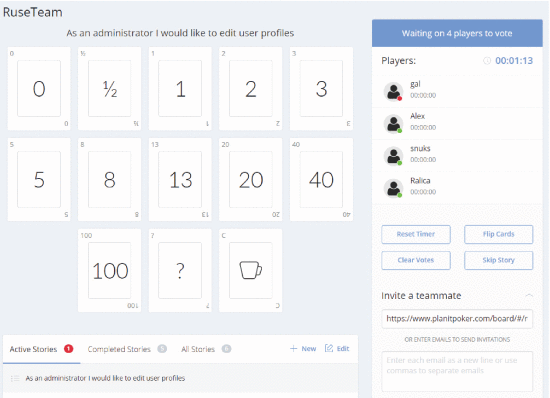
\includegraphics[width=0.5\textwidth]{planitpoker.png}
\caption{Planitpoker.com}
\label{fig:planitpoker}
\end{figure}

\section{Výhody a nevýhody gamifikácie}

\section{Štatistika}

\section{Záver}

\quad
\newpage

\bibliography{literatura}
\bibliographystyle{plain}
\end{document}
